\documentclass[14pt,oneside]{extarticle}

\usepackage{amsmath}
\usepackage{unicode-math}
\renewcommand{\familydefault}{\rmdefault}
\usepackage{mathtext}
\usepackage{geometry}
\geometry{verbose,lmargin=25mm,rmargin=15mm,tmargin=15mm,bmargin=20mm}
\setcounter{secnumdepth}{3}
\setcounter{tocdepth}{3}
\usepackage{setspace}
\setstretch{1.5}

% Картинки (можно встявлять даже pdf)
\usepackage{graphicx}

% Таблицы
\usepackage{tabularx}
% \setlength{\extrarowheight}{0.3cm}
\renewcommand{\arraystretch}{1.5}
\renewcommand{\tabularxcolumn}[1]{>{\centering\arraybackslash\small}m{#1}}
\newcolumntype{B}{>{\bfseries\small}c}
\newcolumntype{R}{>{\small}c}
%% Because html converters don't know tabularnewline
\providecommand{\tabularnewline}{\\}

\makeatletter
%%%%%%%%%%%%%%%%%%%%%%%%%%%%%% Textclass specific LaTeX commands.
\numberwithin{figure}{section}
\numberwithin{table}{section}
\numberwithin{equation}{section}
\makeatother

% Абзацный отступ = 1.25см
\usepackage{indentfirst}
\setlength\parindent{12.5mm}

% Пакет для содержания
\usepackage{tocloft}

% Команда для специальных разделов (введение, обзор литературы, etc)
% Не нумеруются в содержании, по уровню вложенности: 
\newcommand{\specialsection}[1]{
    \phantomsection
    \bigskip\smallskip\hspace{-13.8mm}
    \normalfont\fontsize{18}{18}\textbf{#1}
    \par\bigskip\normalfont\normalsize
    \addcontentsline{toc}{section}{#1}
}

% Размеры заголовков разделов и подразделов
\usepackage{titlesec}
% Раздел: 18pt, добавляем слово "Глава"
\titleformat{\section}
{\fontsize{18}{18}\bfseries}{
\hspace{-1.5mm}Глава \thesection. \hskip-1em}{1em}{}
% Подраздел: 16pt
\titleformat{\subsection}
{\fontsize{16}{16}\bfseries}{\hspace{-0.2mm}\thesubsection}{1em}{}

% Содержание
% Выравнивание заголовка по центру (да, да, с отступом слева)
% т.к. окружение center и \centering не работают
\renewcommand{\cfttoctitlefont}{\hspace{0.35\textwidth} \bfseries\Large}
% \renewcommand{\cftbeforetoctitleskip}{3em}
% Слово "Глава" в содержании
\renewcommand{\cftsecpresnum}{Глава\space}
\newlength\mylength
\settowidth\mylength{\cftsecpresnum}
\addtolength\cftsecnumwidth{1.5\mylength}
% Строки с точками
\renewcommand{\cftsecleader}{\cftdotfill{\cftdotsep}}
% Точки после цифр в в содержании
\renewcommand{\cftsecaftersnum}{.}
\renewcommand{\cftsubsecaftersnum}{.}
% Подровнять subsection под точку главы
% (если глав будет больше десяти, будет чуть хуже)
\setlength{\cftsubsecindent}{2em}
% Интервал глав
\setlength{\cftbeforesecskip}{3pt}

\renewcommand{\cftsecpagefont}{\normalfont}

\usepackage[russian]{babel}
\usepackage{fontspec}
\setmainfont{Times New Roman}
\setmathfont{TeX Gyre Termes Math}
\usepackage{csquotes}

% Пакет, реализующий гиперссылки. Никакого расскрашивания
\usepackage[colorlinks=false,unicode=true,hidelinks]{hyperref}

\newcommand{\ITEM}{\vspace{-0.2cm}\item}
\newcommand{\MList}[1]{\par\begin{itemize}#1\end{itemize}}
\newcommand{\NList}[1]{\par\begin{enumerate}#1\end{enumerate}}

% Шрифт подписи (caption) = 12pt
% (Повезло, что small как раз равен 12pt)
\usepackage[font=small,labelfont=bf]{caption}

% Пакет, который позволяет собирать один документ TeX из нескольких
\usepackage{import}

%Библиография
\usepackage[
    backend=biber,
    %citestyle = alphabetic, 
    %bibstyle = ieee-alphabetic,  
    %sortlocale=en_US,
    sorting=none,
    backref=true,
    hyperref=true,
    style=numeric,%style=alphabetic,
    defernumbers=true,
    isbn=false,
    autolang=none,
    %eid=true,
    doi=false,
    %series=true,
    eprint=false,
    bibencoding = utf8
]{biblatex} %Imports biblatex package

\renewbibmacro{volume+number+eid}{%
    \printfield{volume}%
    \setunit{\addcomma\space}%
    \printfield{number}%
    \printfield{eid}}

\renewbibmacro{in:}{\space}

\DeclareFieldFormat[article]{volume}{{том}\space#1}
\DeclareFieldFormat[article]{number}{{номер}\space#1\addcomma}

\DefineBibliographyStrings{russian}{%
    phdthesis = {диссертация}%
}

\addbibresource{literature.bib} %Import the bibliography file

% Подсветка кода (все стили в файле)
\usepackage{color}
\usepackage{listings}
\definecolor{GrayCodeBlock}{RGB}{248,252,255}
\definecolor{BlackText}{RGB}{41,75,102}
\definecolor{RedTypename}{RGB}{182,86,17}
\definecolor{GreenString}{RGB}{96,172,57}
\definecolor{PurpleKeyword}{RGB}{184,84,212}
\definecolor{GrayComment}{RGB}{100,100,100}
\definecolor{GoldDocumentation}{RGB}{180,165,45}

\lstset{
    columns=fullflexible,
    keepspaces=true,
    frame=single,
    framesep=0pt,
    framerule=0pt,
    framexleftmargin=4pt,
    framexrightmargin=4pt,
    framextopmargin=5pt,
    framexbottommargin=3pt,
    xleftmargin=4pt,
    xrightmargin=4pt,
    backgroundcolor=\color{GrayCodeBlock},
    basicstyle=\ttfamily\small\color{BlackText},
    keywordstyle=\color{PurpleKeyword},
    ndkeywordstyle=\color{RedTypename},
    comment=[l][\color{GrayComment}\slshape]{//},
    morecomment=[s][\color{GrayComment}\slshape]{/*}{*/},
    morecomment=[s][\color{RedTypename}]{\#![}{]},
    morecomment=[s][\color{RedTypename}]{\#[}{]},
    stringstyle=\color{GreenString},
    string=[b]"
}

\lstdefinelanguage{rust}
{
    keywords={
        true,false,
        unsafe,async,await,move,
        use,pub,crate,super,self,mod,
        struct,enum,fn,const,static,let,mut,ref,type,impl,dyn,trait,where,as,
        break,continue,if,else,while,for,loop,match,return,yield,in
    },
    ndkeywords={
        bool,u8,u16,u32,u64,u128,i8,i16,i32,i64,i128,char,str,
        Self,Option,Some,None,Result,Ok,Err,String,Box,Vec,Rc,Arc,Cell,RefCell,HashMap,BTreeMap,
        macro_rules
    },
    comment=[l][\color{GrayComment}\slshape]{//}
}


\begin{document}

\newgeometry{left=30mm, top=20mm, right=15mm, bottom=20mm, nohead, nofoot}
\begin{titlepage}
\begin{center}
Министерство высшего образования и науки Российской федерации

Федеральное государственное автономное \\образовательное учреждение высшего образования

\textbf{<<Национальный исследовательский ядерный университет}
\textbf{<<МИФИ>>}

\vspace{25mm}

\textbf{\textit{\large Фамилия Имя Отчество}} \\[8mm]
% Название
\textbf{\large Выпускная квалификационная работа}\\[3mm]
\textbf{\textit{\large Название работы}}

\vspace{10mm}
Уровень образования: бакалавриат / магистратура\\
Направление 11.04.04 «Электроника и наноэлектроника»\\
Образовательная программа
«Наноэлектроника, спинтроника и фотоника»

\vspace{15mm}

% Научный руководитель, рецензент
\begin{flushleft}
\textbf{Выпускник:} Фамилия И.О.

\hspace{10cm} \textit{Подпись}: \space \hrulefill

\textbf{Научный руководитель:} 

к.ф.-м.н., доцент кафедры физики конденсированных сред

ИНТЭЛ НИЯУ МИФИ, Фамилия И.О.

\hspace{10cm} \textit{Подпись}: \space \hrulefill

\textbf{И.о. заместителя заведующего кафедрой:} 

д.ф.-м.н., профессор кафедры физики конденсированных сред 

ИНТЭЛ НИЯУ МИФИ, Никитенко В.Р.

\hspace{10cm} \textit{Подпись}: \space \hrulefill \space
\end{flushleft}

\vfill 

{Москва}
\par{\the\year{} г.}
\end{center}
\end{titlepage}
% Возвращаем настройки geometry обратно (то, что объявлено в преамбуле)
\restoregeometry
% Добавляем 1 к счетчику страниц ПОСЛЕ titlepage, чтобы исключить 
% влияние titlepage environment
\addtocounter{page}{1}


% Содержание
\tableofcontents
\pagebreak

% ============================================
% ВВЕДЕНИЕ
% ============================================
\specialsection{Введение}

Современное развитие нанотехнологий требует всё более точного контроля над структурой и формой наносистем. Особый интерес в этой области вызывают низкоразмерные квантовые структуры, такие как квантовые точки, нанонити и кольца. Среди них квантовые кольца выделяются своей замкнутой топологией и ярко выраженными квантовыми эффектами, включая эффект Ахаронова–Бома, пространственное разделение электронов и дырок, а также высокую чувствительность к внешним полям. Эти свойства делают кольцевые структуры перспективными кандидатами для использования в квантовых сенсорах, криптографии, системах хранения информации и лазерах на основе межзонных переходов~\cite{jin2010}.

Создание таких структур возможно с помощью различных подходов, включая рост по механизму Штрански–Крастанова, частичное осаждение и отжиг, но одним из наиболее гибких и управляемых методов является капельная эпитаксия. Эта технология была предложена Koguchi и соавторами в 1991 году~\cite{koguchi1991} и позволяет формировать трёхмерные наноструктуры без необходимости напряжённого слоя. Метод заключается в осаждении капель материала группы III (например, Ga) в вакуумной камере молекулярно-лучевой эпитаксии, после чего они преобразуются в кристаллические структуры за счёт воздействия атомов группы V (например, As).

Одним из ключевых преимуществ капельной эпитаксии является широкий диапазон управляемых форм, включая симметричные точки, вытянутые кольца, чашеобразные структуры и полые оболочки. Тем не менее, такие формы получаются не всегда: результаты роста чувствительны к условиям, включая температуру подложки, величину потока мышьяка, временные интервалы подачи компонентов и характеристики самой капли (объём, радиус, контактный угол). В работе~\cite{zhou2013} показано, что незначительные изменения этих параметров приводят к различным морфологиям кольца — от замкнутого симметричного обода до слабо выраженной асимметричной структуры. Аналогичную чувствительность обнаружили и Rastelli и соавт.~\cite{rastelli2004}, исследовавшие переход от квантовой точки к кольцу при частичном пассивировании и отжиге.

Формирование кольца из капли — это сложный физико-химический процесс, в котором участвуют: диффузия Ga и As по поверхности подложки, реакция между ними с образованием кристаллической решётки, десорбция мышьяка в вакуум, уменьшение радиуса капли по мере отдачи атомов Ga, а также геометрические эффекты, связанные с капельным углом и распределением давления.

Понимание этих процессов невозможно без надёжной количественной модели. Качественные гипотезы, основанные на стационарном потоке или равномерной подаче атомов, не позволяют объяснить наблюдаемое разнообразие форм. Здесь важна локальность потока атомов Ga — он сконцентрирован вблизи поверхности капли. Пространственная и временная изменчивость этого профиля напрямую влияет на геометрию кольца.

На практике такое моделирование имеет прикладное значение: оно позволяет прогнозировать форму кольца до проведения эксперимента, оптимизировать параметры роста, а также адаптировать технологию под целевые оптические и электронные свойства. Более того, численная модель может быть использована для решения обратной задачи — подбора условий роста под заданную морфологию.

Таким образом, актуальность настоящей работы определяется необходимостью построения и исследования физико-математической модели роста квантовых колец методом капельной эпитаксии, учитывающей локализованный поток атомов Ga, диффузию, реакционную кинетику, изменение формы капли и влияние внешних параметров роста.

\specialsection{Цель и задачи}

\textbf{Цель исследования} заключается в разработке и реализации численной модели капельной эпитаксии квантовых колец с учётом пространственно-временной эволюции радиуса капли и распределения концентраций атомов Ga и As, а также в анализе влияния условий роста на морфологию конечной структуры. Дополнительно целью является программная реализация модели и визуализация полученных результатов.

Для достижения указанной цели были поставлены следующие задачи:

\begin{enumerate}
  \item Исследовать физические механизмы формирования квантовых колец в рамках капельной эпитаксии, включая диффузию, десорбцию, реакционную кинетику и геометрию капли.
  \item Построить математическую модель на основе системы дифференциальных уравнений, описывающих поведение концентраций Ga и As и изменение радиуса капли во времени.
  \item Разработать численный алгоритм на основе конечно-разностной схемы (схемы Эйлера) для решения системы уравнений.
  \item Реализовать алгоритм в виде программы на языке Rust, включая:
  \begin{itemize}
    \item дискретизацию сетки по времени и пространству;
    \item вычисление профиля высоты кольца;
    \item сохранение результатов в виде файлов концентраций, высот и радиуса.
  \end{itemize}
  \item Провести серию численных экспериментов для анализа влияния параметров роста (температура, флюкс мышьяка, ширина гауссова распределения, угол смачивания) на форму кольца.
  \item Сравнить качественные характеристики полученных профилей с экспериментальными данными из научной литературы.
\end{enumerate}

% ============================================
% ГЛАВА 1
% ============================================

\pagebreak
\section{Теоретические основы капельной эпитаксии квантовых колец}

\subsection{Капельная эпитаксия: физика и стадии роста}

Капельная эпитаксия является разновидностью молекулярно-лучевой эпитаксии и используется для формирования наноразмерных структур — квантовых точек, колец, а также более сложных ансамблей. Основной особенностью метода является пространственное и временное разделение подачи атомов III и V групп. Это позволяет управлять процессом образования капель, их трансформацией и последующей кристаллизацией~\cite{gurioli2021, koguchi1991}.

Процесс капельной эпитаксии условно делится на несколько этапов:

\begin{enumerate}
    \item \textbf{Формирование капли.} На предварительно подготовленную поверхность подложки (например, GaAs) осаждаются атомы элемента III группы (чаще всего — галлия) при выключенном потоке V-группы. В отсутствие аннигиляции или немедленной реакции атомы Ga собираются в жидкие капли, распределяющиеся по поверхности в зависимости от температуры, плотности потока и состояния подложки.
    
    \item \textbf{Кристаллизация.} После формирования капли открывается поток мышьяка, и начинается стадия кристаллизации. Атомы As взаимодействуют с жидкой каплей Ga, образуя твердую фазу GaAs. На этом этапе большое значение имеет конкуренция между двумя путями роста: прямой реакцией внутри капли и кристаллизацией на поверхности в результате диффузии атомов.
    
    \item \textbf{Рост структуры.} В зависимости от соотношения этих процессов, геометрии капли и внешних условий может быть реализован рост квантовой точки, кольца или их комбинации. Так, преобладание поверхностной диффузии атомов Ga ведёт к формированию кольца, тогда как внутренняя реакция способствует образованию компактной точки.
    
    \item \textbf{Дополнительная обработка.} При необходимости структура может быть подвергнута термическому отжигу или заращиванию покровным слоем, что изменяет её морфологию, симметрию и оптические свойства. Например, частичный отжиг может привести к перераспределению материала и трансформации точки в кольцо.
\end{enumerate}

Морфология образующихся структур чувствительна к ряду технологических параметров: температуре подложки, интенсивности и длительности потока компонентов, времени экспозиции, а также к типу и ориентации подложки. Это делает капельную эпитаксию не только удобным, но и гибким инструментом для целенаправленного синтеза наноструктур с заданными свойствами~\cite{sibirmovskiy2014}.

Стадии капельной эпитаксии наглядно представлены на схематическом изображении, заимствованном из статьи~\cite{gurioli2021} (рис.~\ref{fig:gurioli1}). На нём показан процесс формирования капель, возможные пути кристаллизации и типичные формы наноструктур.

\begin{figure}
    \begin{center}
        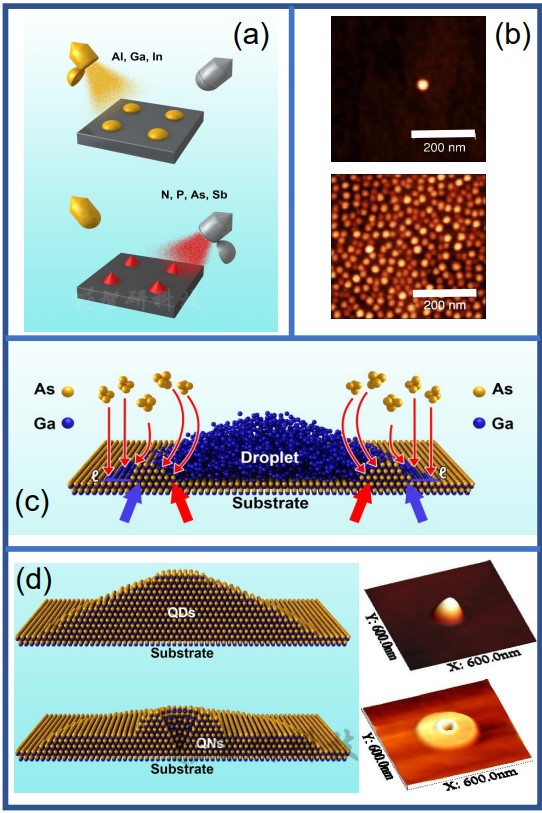
\includegraphics[width=11cm]{images/gurioli_fig1.png}
        \caption{\label{fig:gurioli1}
            Стадии капельной эпитаксии (воспроизведено из~\cite{gurioli2021}): (a) схема последовательного осаждения атомов III и V группы, (b) AFM-изображения капель с различной плотностью, (c) два механизма роста — поглощение атомов As каплей и диффузия Ga наружу, (d) формирование квантовой точки или кольца в зависимости от доминирующего механизма.}
    \end{center}
\end{figure}

Дополнительно, на рис.~\ref{fig:zhou1} представлена последовательность реальных SEM-изображений, иллюстрирующая трансформацию капли Ga во времени под действием потока As, в том числе образование двойного кольца. Эти данные наглядно подтверждают описанный выше механизм.

\begin{figure}
    \begin{center}
        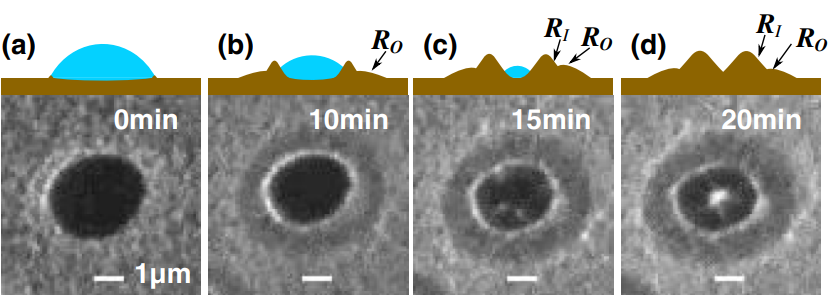
\includegraphics[width=11cm]{images/Zhou1-Firgure1.png}
        \caption{\label{fig:zhou1}
            Эволюция капли Ga и формирование квантового кольца во времени при капельной эпитаксии. Изображения получены методом MEM. Виден переход от капли к юбкообразной структуре и далее к двойному кольцу. Воспроизведено из~\cite{zhou2013}.}
    \end{center}
\end{figure}

\subsection{Квантовые кольца: геометрия, свойства, эффекты}

Квантовые кольца (КК) — это наноструктуры с тороидальной симметрией и выраженным центральным отверстием, отличающиеся от квантовых точек своей геометрией и спектром состояний. Такая топология существенно влияет на свойства локализованных в кольце электронов и дырок. В отличие от точек, где частицы локализуются в центре, в кольце они прижаты к периферии, что приводит к целому ряду квантовых эффектов.

Один из наиболее ярких эффектов — это эффект Ааронова–Бома, при котором энергетические уровни квантового кольца осциллируют в зависимости от магнитного потока, проходящего через его центр. Уравнение для энергии носителя в кольце радиуса $r$ имеет вид:

\[
E_M = \frac{\hbar^2}{2m^* r^2} \left( M + \frac{\Phi}{\Phi_0} \right)^2,
\]

где $M$ — магнитное квантовое число, $m^*$ — эффективная масса, $\Phi$ — магнитный поток, $\Phi_0 = h/e$ — квант потока.

Наличие топологического отверстия также влияет на пространственное распределение плотности состояний, запрещая плотную локализацию в центре и изменяя характер волновых функций. Это приводит к специфическим оптическим переходам: изменениям в ширине линии фотолюминесценции, поляризационной анизотропии, а также чувствительности к направлению магнитного поля.

Согласно экспериментальным данным~\cite{sibirmovskiy2018}, кольца на основе GaAs/AlGaAs демонстрируют необычную температурную зависимость фотолюминесценции: при нагревании от 20 до 70 К интенсивность ФЛ растёт, а ширина линии уменьшается, что связывается с термоактивацией носителей и неоднородной формой кольца. Кроме того, благодаря высокой симметрии кольцевой формы, КК демонстрируют слабо выраженную поляризацию испускаемого света, что делает их удобными для задач квантовой фотоники.

Энергетические и оптические свойства КК зависят от их геометрических параметров — внешнего и внутреннего радиусов, толщины, глубины. Геометрия, в свою очередь, может быть определена, например, методом атомно-силовой микроскопии. На рис.~\ref{fig:elborg2} представлен AFM-изображение одиночного квантового кольца, полученного в работе~\cite{elborg2017}.

\begin{figure}
    \begin{center}
        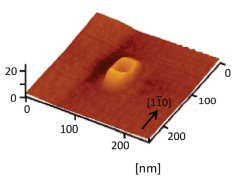
\includegraphics[width=11cm]{images/elborg_fig2.png}
        \caption{\label{fig:elborg2}
            AFM-изображения одиночного квантового кольца (вверху) и кольца с точкой в центре (внизу), полученных методом капельной эпитаксии. Воспроизведено из работы~\cite{elborg2017}.}
    \end{center}
\end{figure}

Квантовые кольца находят применение в квантовой криптографии, в качестве однофотонных источников, а также в схемах логических вентилей, использующих спиновые и орбитальные степени свободы. Их особые геометрические и магнитные свойства делают их также перспективными для реализации твердотельных квантовых битов.

\subsection{Влияние условий роста на морфологию квантовых колец}

Морфология квантовых колец, формируемых методом капельной эпитаксии, определяется множеством взаимосвязанных параметров. Помимо температуры подложки и потока мышьяка, большое значение имеют: объём капли, ориентация кристаллической подложки, режим подачи компонентов, параметры десорбции и свойства мокрого слоя. Управление этими факторами позволяет синтезировать кольца с заданной формой, размерами и симметрией.

Одним из наиболее исследованных параметров является температура подложки. При низких температурах ($T < 250\,^{\circ}\mathrm{C}$) ограниченная диффузия атомов Ga приводит к формированию компактных точек или толстостенных колец. При увеличении температуры ($T \approx 300\,^{\circ}\mathrm{C}$) диффузия усиливается, что способствует расширению кольца и образованию симметричной структуры. Однако при слишком высоких температурах ($T > 330\,^{\circ}\mathrm{C}$) доминирует десорбция мышьяка, что может привести к неравномерной кристаллизации и даже исчезновению кольца~\cite{sibirmovskiy2014,vasilevskiy2013}.

Интенсивность потока мышьяка (или эффективное давление As$_4$) регулирует скорость кристаллизации. Высокий поток ведёт к мгновенному насыщению капли As и образованию точек. Напротив, при умеренном или ступенчатом потоке As возможно последовательное формирование двойных или концентрических колец, как показано в работах Zhou et al.~\cite{zhou2013} и Fan и Ma~\cite{fan2023}.

\begin{figure}
    \begin{center}
        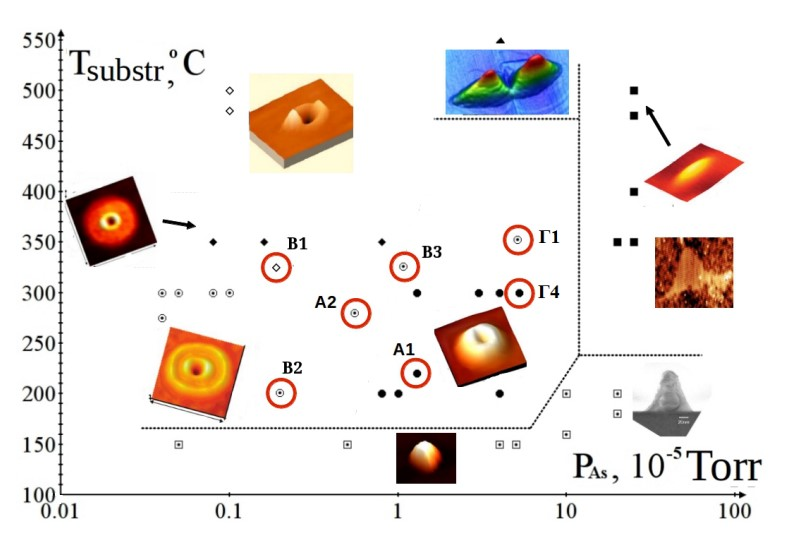
\includegraphics[width=14cm]{images/morphology_map.png}
        \caption{\label{fig:morph_map}
            Морфология квантовых колец GaAs/AlGaAs в зависимости от температуры подложки и давления мышьяка. Изображения структур заимствованы из работ~\cite{mano2005nano, koguchi2005growth, vasilevskiy2013}.}
    \end{center}
\end{figure}

Схожие результаты были получены в недавней обзорной работе Fan и Ma~\cite{fan2023}, где показано, как изменяются формы GaAs наноструктур (точки, кольца, двойные кольца, углубления) при варьировании температуры и потока As. При 150 °C формируются точки, при 200 °C — кольца, а при 300 °C наблюдаются двойные кольца и кольцевые углубления. Аналогично, при фиксированной температуре изменение потока As также приводит к трансформации форм.

\begin{figure}
    \begin{center}
        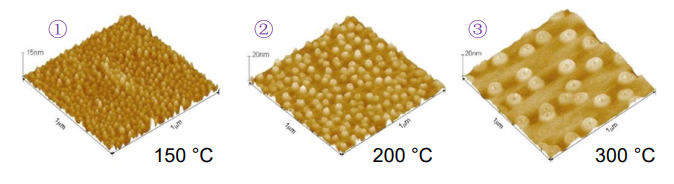
\includegraphics[width=11cm]{images/fanma_fig2e_left.png}
        \caption{\label{fig:fanma_temp}
            Изменение формы квантовых колец GaAs в зависимости от температуры. Воспроизведено из~\cite{fan2023}, рис.~2(e).}
    \end{center}
\end{figure}

\begin{figure}
    \begin{center}
        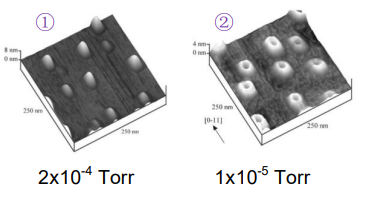
\includegraphics[width=11cm]{images/fanma_fig2e_right.png}
        \caption{\label{fig:fanma_pressure}
            Изменение формы квантовых колец GaAs в зависимости от давления мышьяка. Воспроизведено из~\cite{fan2023}, рис.~2(f).}
    \end{center}
\end{figure}

Помимо температуры подложки и потока мышьяка, на морфологию квантовых колец существенное влияние оказывают и другие параметры роста. К ним относятся:

\begin{itemize}
    \item \textbf{Объём капли Ga.} Определяет форму и ширину кольца. При малом объёме формируются узкие симметричные кольца, при увеличенном — кольца с размытыми границами или асимметрией. Существенное влияние оказывает начальный радиус и масса капли~\cite{zhou2013}.

    \item \textbf{Ориентация подложки.} На подложках GaAs(001) и GaAs(111) наблюдаются различия в симметрии кольцевых структур. Анизотропия поверхностной энергии и направленности диффузии приводит к вытягиванию кольца вдоль кристаллографических осей~\cite{elborg2017}.

    \item \textbf{Наличие смачивабщего слоя.} Если до или во время кристаллизации присутствует остаточный слой Ga или GaAs, он может «заполнять» центр кольца, делая профиль менее глубоким. В его отсутствие кольцо формируется с резкой ямой в центре~\cite{sibirmovskiy2014}.

    \item \textbf{Режим подачи мышьяка.} При непрерывной подаче формируются одиночные кольца, а при ступенчатой или импульсной — двойные и многокольцевые структуры. Режим подачи влияет на скорость кристаллизации и изменение границ капли~\cite{wang2022}.

    \item \textbf{Десорбция мышьяка.} При повышенных температурах атомы As быстро десорбируются с поверхности до завершения реакции, что может привести к неравномерной или частично разрушенной кольцевой морфологии~\cite{fan2023}.
\end{itemize}

Таким образом, морфология квантовых колец — это результат тонкого баланса между параметрами роста, диффузией, реакцией и десорбцией. Только комплексное управление этими условиями позволяет воспроизводимо получать наноструктуры с нужной формой и функциональностью.

\subsection{Современные подходы к моделированию роста квантовых колец}

Моделирование роста квантовых колец методом капельной эпитаксии остаётся активно развивающимся направлением, в котором используется широкий спектр физических и численных подходов. В данной части представлены основные классы моделей, применяемые в литературе, с анализом их возможностей и ограничений.

\subsubsection*{Модели на основе уравнений диффузии и химической реакции}
Один из наиболее распространённых подходов основан на описании эволюции поверхностных концентраций компонентов III и V групп с помощью реакционно-диффузионных уравнений. Такие модели позволяют анализировать пространственное распределение атомов и воспроизводить морфологию кольца. Классическим примером является модель, предложенная в работе Zhou et al.\cite{zhou2013}, в которой учитываются диффузия атомов Ga и As, их взаимодействие, а также влияние параметров роста. Модель хорошо воспроизводит профиль кольца, но не учитывает динамическое изменение радиуса капли, что ограничивает её применимость на длительных временах. На рис.\ref{fig:zhou_profiles} показано соответствие между профилем кольца, полученным в расчёте, и экспериментальными AFM-данными.

\begin{figure}
    \begin{center}
        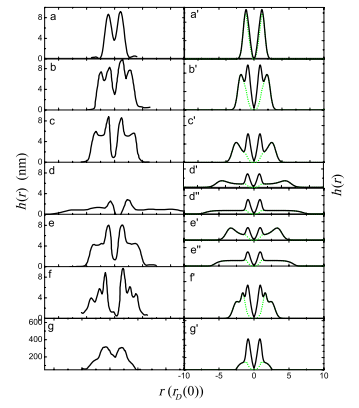
\includegraphics[width=11cm]{images/zhou_profiles.png}
        \caption{\label{fig:zhou_profiles}
            Сравнение экспериментальных (слева) и рассчитанных (справа) профилей высоты кольцевых структур GaAs. Воспроизведено из~\cite{zhou2013}, рис.~4.}
    \end{center}
\end{figure}

\subsubsection*{Кинетические модели нуклеации и эволюции капель}
Другим направлением являются модели, описывающие образование и эволюцию капель на подложке. Они фокусируются на стадиях нуклеации, росте и слиянии капель, а также на влиянии температуры и плотности потока. Модель Dubrovskii et al.\cite{dubrovskii2021} представляет собой систему обыкновенных дифференциальных уравнений для плотностей мономеров, капель и критического размера. Она позволяет количественно описать начальную стадию формирования кольца, однако не рассматривает морфологию полученной структуры. На рис.\ref{fig:dubrovskii_model} показана временная эволюция параметров нуклеации согласно расчётам данной модели.

\begin{figure}
    \begin{center}
        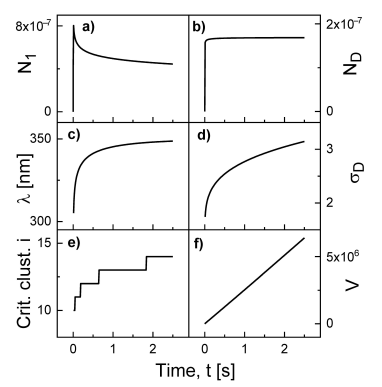
\includegraphics[width=11cm]{images/dubrovskii_fig2.png}
        \caption{\label{fig:dubrovskii_model}
            Временная эволюция параметров нуклеации и роста капли: (a--f) — плотность мономеров, плотность капель, длина диффузии, число захвата, критический размер, объём капли. Воспроизведено из~\cite{dubrovskii2021}, рис.~2.}
    \end{center}
\end{figure}

\subsubsection*{Модели на основе метода Монте-Карло}
Для описания сложной кинетики роста на атомарном уровне применяются модели на основе кинетического Монте-Карло. Они позволяют учитывать локальные процессы осаждения, поверхностной диффузии и кристаллизации. Примером служит модель Shwartz et al.\cite{shwartz2018}, в которой смоделировано образование кольца с учётом направления поступления атомов As, перераспределения Ga и влияния геометрии капли. Такие модели хорошо воспроизводят эволюцию формы, но являются вычислительно затратными и трудны для параметрического анализа. На рис.\ref{fig:shwartz4} приведены последовательные конфигурации кольца на различных стадиях роста.

\begin{figure}
    \begin{center}
        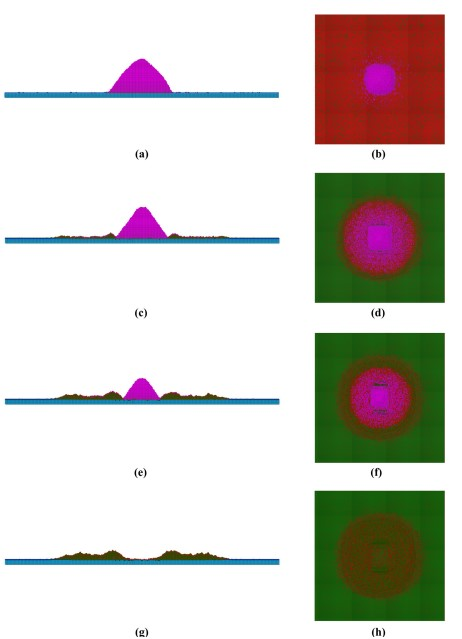
\includegraphics[width=11cm]{images/shwartz_fig4.png}
        \caption{\label{fig:shwartz4}
            Эволюция морфологии кольца в модели Монте-Карло. Слева — поперечные сечения, справа — вид сверху. Капля Ga обозначена фиолетовым, GaAs — коричневым. Воспроизведено из~\cite{shwartz2018}, рис.~4.}
    \end{center}
\end{figure}

\subsubsection*{Сравнительный анализ подходов}
Все рассмотренные модели акцентируют внимание на различных аспектах роста кольца. Диффузионно-реакционные модели эффективны при анализе морфологии, но чувствительны к выбору граничных условий. Кинетические уравнения нуклеации хорошо описывают начальную стадию, но не дают информации о форме. Модели Монте-Карло подходят для анализа атомарных механизмов, но требуют большого объёма вычислений.

Для целей данной работы необходимо было объединить преимущества разных подходов: описать как пространственную структуру концентраций, так и изменение геометрии капли во времени. Поэтому была выбрана гибридная модель, сочетающая диффузию, химию и динамику радиуса — подробнее она представлена в следующем разделе.

\subsection{Обоснование выбора подхода к моделированию}

Анализ существующих моделей показывает, что каждая из них решает строго ограниченную задачу: описывает либо морфологию кольца при фиксированных условиях, либо начальную стадию нуклеации капли, либо пространственно-атомарную кинетику. Однако ни одна из них не объединяет в себе:

\begin{itemize}
  \item динамическое изменение радиуса капли;
  \item пространственно-временное распределение концентраций Ga и As;
  \item рост высоты кольца как результат поверхностной реакции;
  \item физически обоснованное распределение потока галлия из капли.
\end{itemize}

В связи с этим в рамках данной работы была разработана модель, сочетающая принципы реакционно-диффузионного описания, приближённое уравнение эволюции радиуса капли, численное описание роста кольца и гауссов профиль потока. Такая постановка позволяет анализировать влияние параметров роста на морфологию кольца и служит основой для построения численной схемы.

Подробное описание модели и всех входящих уравнений приводится в следующей главе.


% ============================================
% ГЛАВА 2
% ============================================
\pagebreak

\section{Физико-математическая модель}

\subsection{Основные уравнения диффузии и реакций}

Процесс формирования кольцевой структуры при капельной эпитаксии можно описывать с помощью реакционно-диффузионной модели в предположении осевой симметрии. Подобные модели применяются в ряде современных исследований~\cite{reyes2013, bietti2020}, позволяя анализировать пространственно-временное распределение компонентов и их взаимодействие на поверхности.

Пусть $c_{\text{Ga}}(r,t)$ и $c_{\text{As}}(r,t)$ — поверхностные концентрации атомов галлия и мышьяка соответственно, зависящие от радиальной координаты $r$ и времени $t$.

Для обоих компонентов учитываются диффузия, поступление вещества (для As — постоянный поток, для Ga — гауссов профиль из капли), а также реакция между ними, приводящая к образованию твёрдой фазы GaAs. Для мышьяка дополнительно учитывается десорбция с поверхности.

Такой подход описан, в частности, в работе~\cite{reyes2013_1}, где предложена численная модель, объединяющая кинетические и диффузионные аспекты. В другом исследовании~\cite{bietti2020} показано, как изменение арсенизации и температуры влияет на соотношение между объёмами GaAs, кристаллизующегося внутри капли и по её границе.

Уравнения системы имеют следующий вид:

\begin{equation}
\frac{\partial C_{Ga}}{\partial t}=D_{Ga}\frac{1}{r}\frac{\partial}{\partial r}\left(r\frac{\partial C_{Ga}}{\partial r}\right)+F_{Ga}\left(r,t\right)-k_{r}C_{Ga}C_{As}
\label{eq:ga_diff}
\end{equation}

\begin{equation}
\frac{\partial C_{As}}{\partial t}=D_{As}\frac{1}{r}\frac{\partial}{\partial r}\left(r\frac{\partial C_{As}}{\partial r}\right)+F_{As}-k_{r}C_{Ga}C_{As}-\frac{C_{As}}{\tau_{As}},
\label{eq:as_diff}
\end{equation}

где:
\begin{itemize}
  \item $D_{\text{Ga}}, D_{\text{As}}$ — коэффициенты поверхностной диффузии;
  \item $\omega$ — коэффициент реакции между атомами Ga и As;
  \item $F_{\text{As}}$ — постоянный поток мышьяка;
  \item $F_{\text{Ga}}(r,t)$ — пространственно и временно зависимый поток галлия;
  \item $\tau_{\text{As}}$ — характерное время испарения мышьяка.
\end{itemize}

\begin{equation}
D_{Ga}=a_{0}^{2}\nu\exp\left(-\frac{E_{Ga}}{kT}\right)
\end{equation}

\begin{equation}
D_{As}=a_{0}^{2}\nu\exp\left(-\frac{E_{As}}{kT}\right)
\end{equation}

Время десорбции мышьяка:

\begin{equation}
\tau_{As}=\frac{1}{\nu}\exp\left(\frac{E_{a}}{kT}\right)
\end{equation}

\begin{equation}
\nu=\frac{kT}{\pi\hbar}
\end{equation}

Модель использует приближение сплошной среды, что оправдано для масштабов порядка десятков нанометров. Она позволяет изучать влияние параметров роста на морфологию кольца в рамках эффективной численной реализации.

Модель задаётся на интервале $r \in [0, R_\infty]$ с осевой симметрией. Поверхностные концентрации атомов $C_{\text{Ga}}(r,t)$ и $C_{\text{As}}(r,t)$ описываются уравнениями~\eqref{eq:ga_diff}–\eqref{eq:as_diff}, и для их корректного численного решения необходимо задать начальные и граничные условия.

\subsubsection*{Начальные условия}

На начальный момент времени ($t = 0$): 

\begin{equation}
C_{Ga}\left(r,0\right)=0, \qquad
C_{As}\left(r,0\right)=0.
\end{equation}

\subsubsection*{Граничные условия}

На правой границе области ($r = R_\infty$) задаются:

\begin{equation}
C_{Ga}\left(R_{\infty},t\right)=0, \qquad
C_{As}\left(R_{\infty},t\right)=F_{As}\tau_{As}.
\end{equation}

\subsection{Распределение потока галлия из капли}

Одним из ключевых элементов модели капельной эпитаксии является описание пространственного распределения потока галлия, поступающего из жидкой капли на подложку. Корректное задание этой функции необходимо для воспроизведения морфологии кольца и скорости роста наноструктуры. Ниже приведено подробное аналитическое построение соответствующего выражения, опирающееся на решение уравнения диффузии с заданными граничными условиями.

Нам требуется дополнительная концентрация атомов Ga на границе капли в соответствии с:

\begin{equation}
\tilde{C}_{Ga}\left(r,t\right)=C_{0}\exp\left(-\frac{\left(r-R_{d}\left(t\right)\right)^{2}}{w^{2}}\right)
\end{equation}

Это приводит к дополнительному потоку, который является нашим единственным источником атомов Ga (рис.~\ref{fig:first}):

\begin{equation}
F_{Ga}\left(r,t\right)=\frac{C_{0}}{\tau_{Ga}\left(t\right)}\exp\left(-\frac{\left(r-R_{d}\left(t\right)\right)^{2}}{w^{2}}\right)
\end{equation}

\begin{figure}
    \begin{center}
        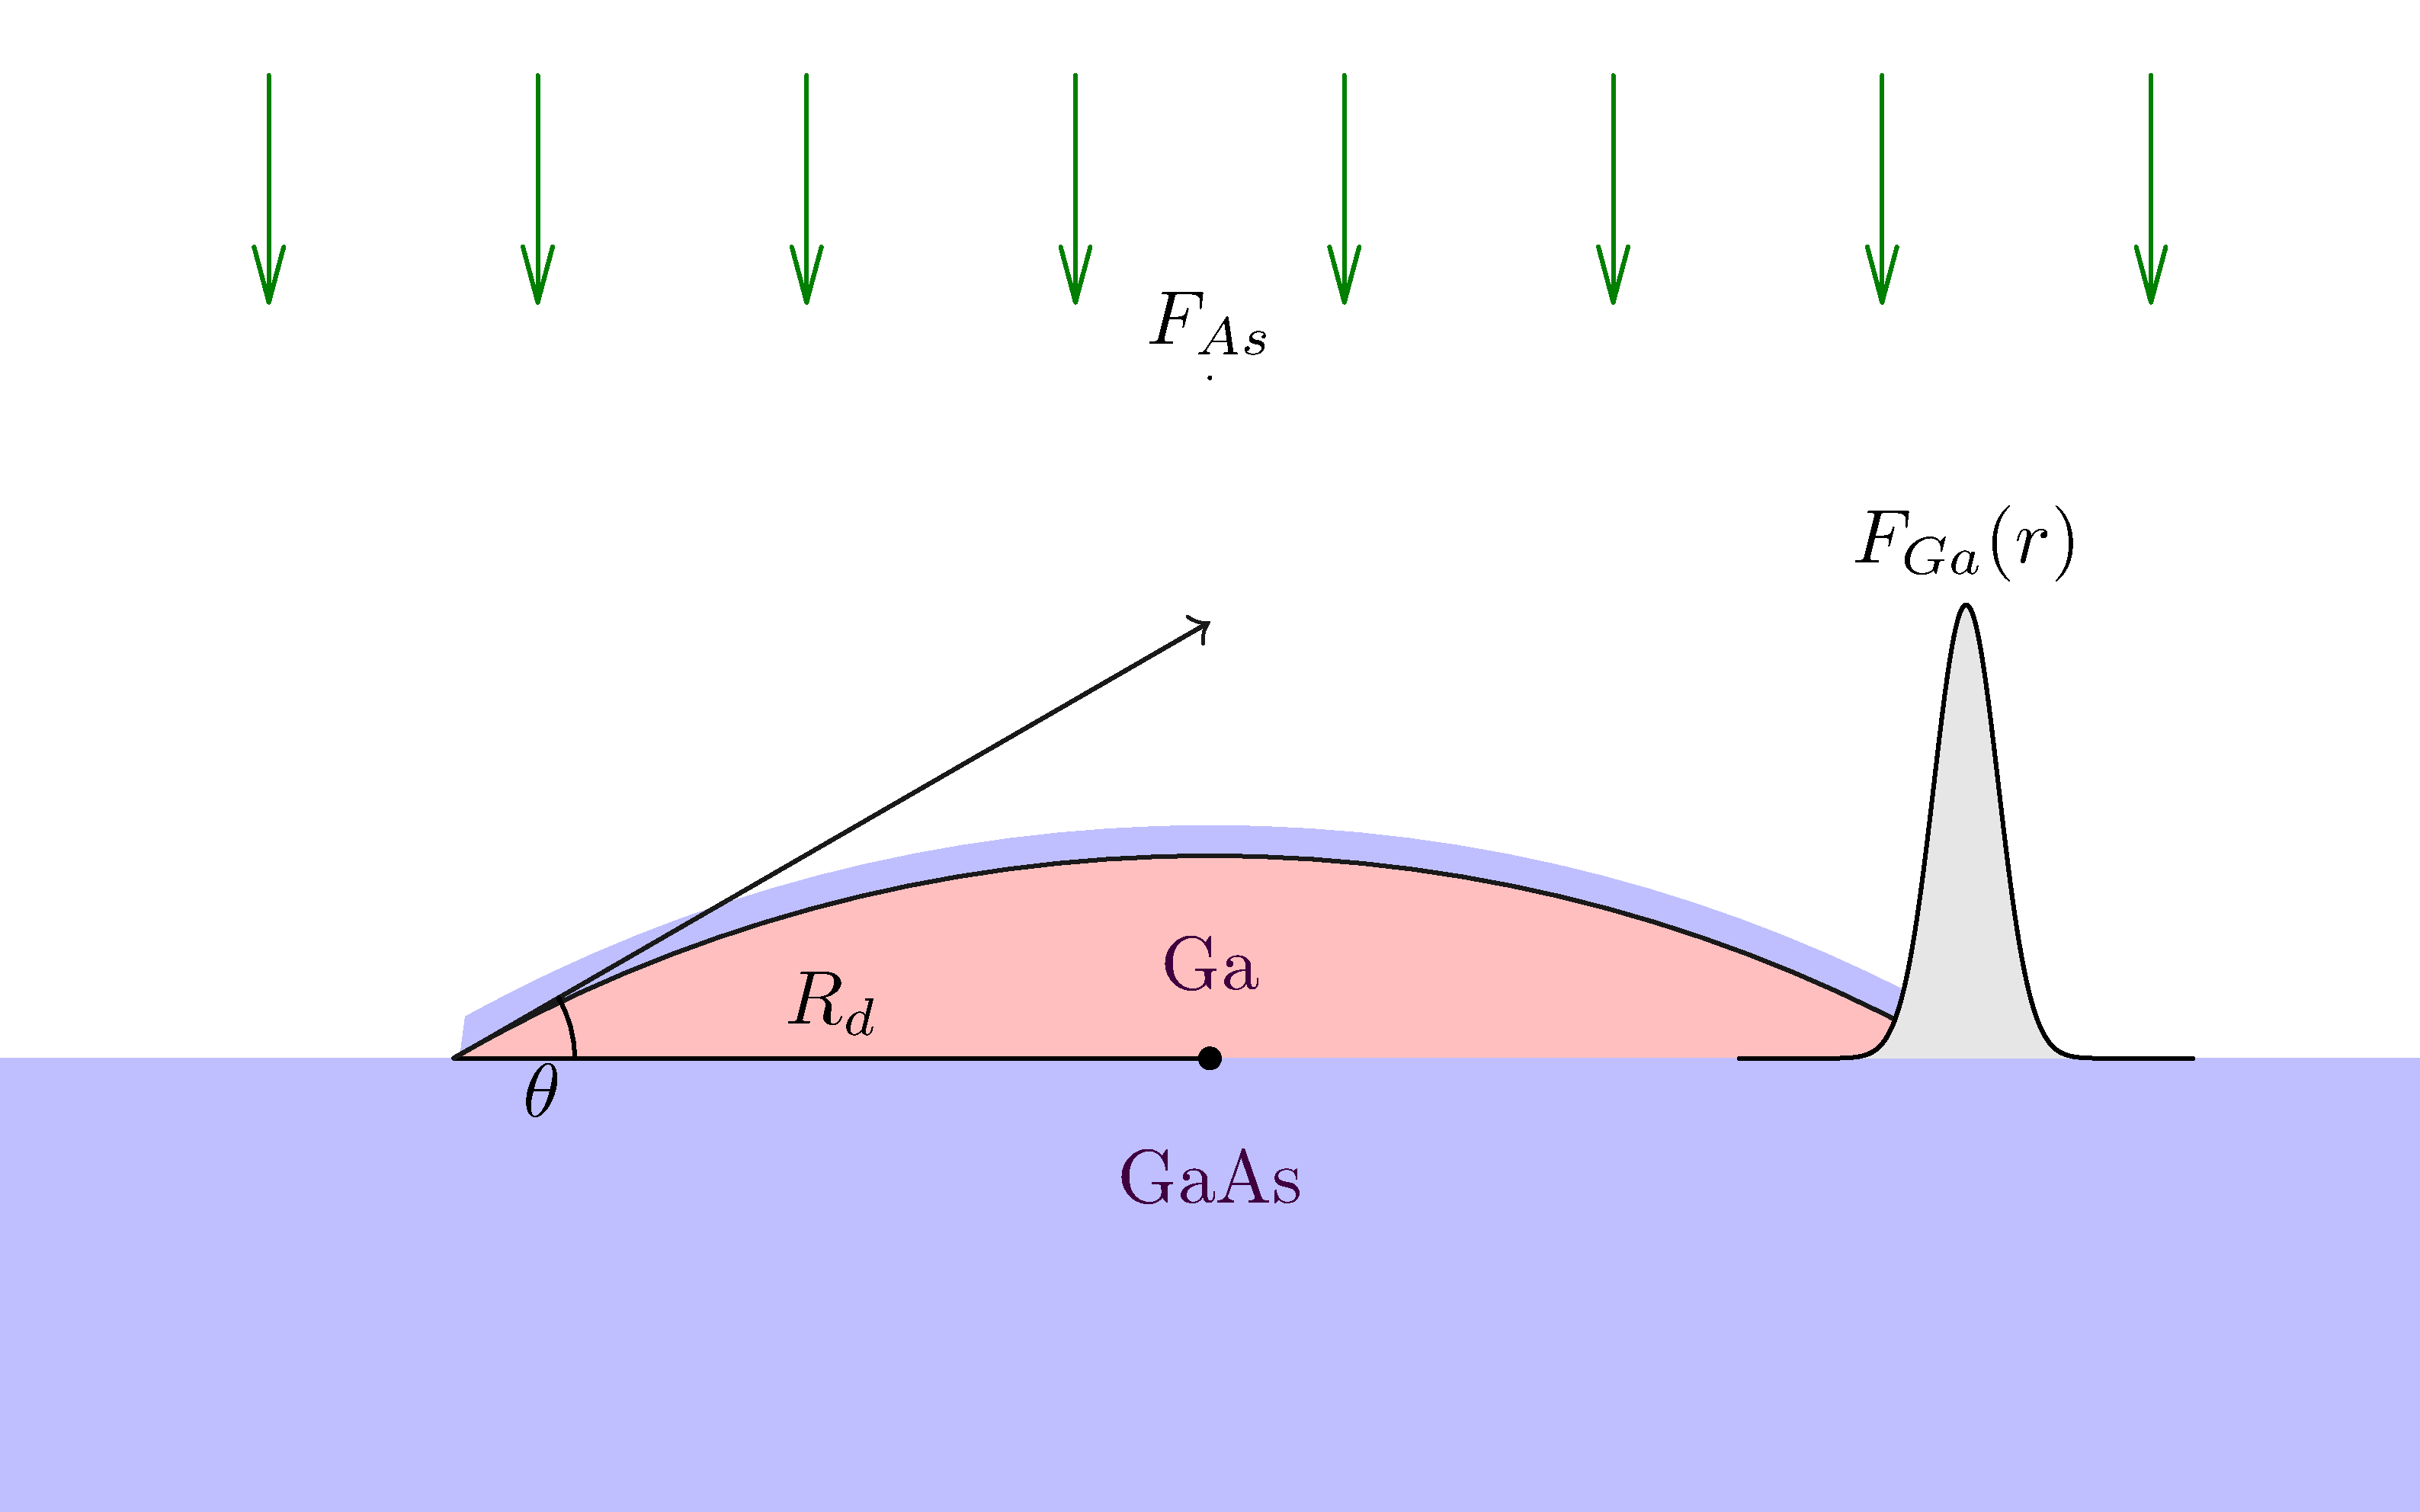
\includegraphics[width=11cm]{images/first.png}
        \caption{\label{fig:first}
        Визуализация потоков вещества Ga}
    \end{center}
\end{figure}

Чтобы найти параметр $\tau_{\text{Ga}}$ (где $w$ — свободное постоянное значение), нам нужно учесть потерю атомов Ga. Для этого мы рассмотрим более простую модель, в которой расчёт выполняется для $r \in [R_{d}, R_{\infty}]$ и присутствует только Ga. Это приводит к следующему уравнению:

\begin{equation}
\frac{\partial C_{Ga}}{\partial t}=D_{Ga}\frac{1}{r}\frac{\partial}{\partial r}\left(r\frac{\partial C_{Ga}}{\partial r}\right)
\end{equation}

\[
C_{\text{Ga}}\left(R_d, t\right) = C_0,
\qquad
C_{\text{Ga}}\left(R_\infty, t\right) = 0
\]

Мы можем решить эту проблему путем разделения переменных или просто рассмотреть стационарное состояние:

\[
\frac{\partial C_{Ga}}{\partial t}=0
\]

Тогда нам нужно решить:

\[
\frac{\partial}{\partial r}\left(r\frac{\partial C_{Ga}}{\partial r}\right)=0
\]

Мы получаем общее решение:

\[
C_{Ga}=A\ln\frac{r}{R_{0}}
\]

Где $A,R_{0}$ - неизвестные константы. Замена граничных условий приводит к:

\[
A\ln\frac{R_{d}}{R_{0}}=C_{0}
\qquad
A\ln\frac{R_{\infty}}{R_{0}}=0
\]

Таким образом, мы получаем:

\[
R_{0}=R_{\infty}
\]

\begin{equation}
A=\frac{C_{0}}{\ln\frac{R_{d}}{R_{\infty}}}
\end{equation}

Из чего следует:

\begin{equation}
C_{Ga}=\frac{C_{0}}{\ln\frac{R_{d}}{R_{\infty}}}\ln\frac{r}{R_{\infty}}
\end{equation}

Теперь нам нужно найти поток от границы капли:

\begin{equation}
J_{Ga}=-D_{Ga}\frac{\partial C_{Ga}}{\partial r}\left(r=R_{d}\right)
\end{equation}

\begin{equation}
\frac{\partial C_{Ga}}{\partial r}\left(r=R_{d}\right)=\frac{C_{0}}{R_{d}\ln\frac{R_{d}}{R_{\infty}}}
\end{equation}

\[
J_{Ga}=-\frac{D_{Ga}C_{0}}{R_{d}\ln\frac{R_{d}}{R_{\infty}}}
\]

Поток положительный (потому что он должен двигаться от капли в направлении r → $R_{infty}$), поэтому мы переписываем его как:

\begin{equation}
J_{Ga}=\frac{D_{Ga}C_{0}}{R_{d}\ln\frac{R_{\infty}}{R_{d}}}>0
\end{equation}

Изменение числа атомов Ga:

\begin{equation}
\frac{dN_{Ga}}{dt}=-2\pi R_{d}J_{Ga}=-2\pi\frac{D_{Ga}C_{0}}{\ln\frac{R_{\infty}}{R_{d}}}
\end{equation}

С другой стороны, в нашей первоначальной задаче мы имеем:

\begin{equation}
\frac{dN_{Ga}}{dt}=-2\pi\int_{0}^{R_{\infty}}F_{Ga}rdr
\end{equation}

\[
-\frac{dN_{Ga}}{dt}=2\pi\frac{C_{0}}{\tau_{Ga}}\int_{0}^{R_{\infty}}\exp\left(-\frac{\left(r-R_{d}\right)^{2}}{w^{2}}\right)rdr=
\]

\[
u=r-R_{d},\qquad r=u+R_{d}
\]

\begin{equation}
=2\pi\frac{C_{0}}{\tau_{Ga}}\int_{-R_{d}}^{R_{\infty}-R_{d}}\exp\left(-\frac{u^{2}}{w^{2}}\right)udu+2\pi\frac{C_{0}R_{d}}{\tau_{Ga}}\int_{-R_{d}}^{R_{\infty}-R_{d}}\exp\left(-\frac{u^{2}}{w^{2}}\right)du
\end{equation}

Благодаря симметрии:

\[
\int_{-R_{d}}^{R_{d}}\exp\left(-\frac{u^{2}}{w^{2}}\right)udu=0
\]

\[
\int_{-R_{d}}^{R_{\infty}-R_{d}}\exp\left(-\frac{u^{2}}{w^{2}}\right)udu=\int_{R_{d}}^{R_{\infty}-R_{d}}\exp\left(-\frac{u^{2}}{w^{2}}\right)udu
\]

\[
-\frac{dN_{Ga}}{dt}=\pi\frac{C_{0}w^{2}}{\tau_{Ga}}\int_{\frac{R_{d}^{2}}{w^{2}}}^{\frac{\left(R_{\infty}-R_{d}\right)^{2}}{w^{2}}}\exp\left(-v\right)dv+2\pi\frac{C_{0}wR_{d}}{\tau_{Ga}}\int_{-\frac{R_{d}}{w}}^{\frac{R_{\infty}-R_{d}}{w}}\exp\left(-v^{2}\right)dv
\]

\begin{equation}
    \begin{split}
    -\frac{dN_{Ga}}{dt} &= \pi \frac{C_{0} w^{2}}{\tau_{Ga}} \left[
    \exp\left(-\frac{R_{d}^{2}}{w^{2}}\right)
    - \exp\left(-\frac{(R_{\infty} - R_{d})^{2}}{w^{2}}\right) \right. \\
    &\quad + \left. \sqrt{\pi} \frac{R_{d}}{w}
    \left\{ \text{erf}\left(\frac{R_{\infty} - R_{d}}{w}\right)
    + \text{erf}\left(\frac{R_{d}}{w}\right) \right\}
    \right]
    \end{split}
\end{equation}
    

Сравнение двух потоков дает нам следующее уравнение:

\[
    \begin{split}
    \frac{D_{Ga}}{\ln\frac{R_{\infty}}{R_{d}}} &= \frac{1}{2} \cdot \frac{w^{2}}{\tau_{Ga}} \left[
    \exp\left(-\frac{R_{d}^{2}}{w^{2}}\right)
    - \exp\left(-\frac{(R_{\infty} - R_{d})^{2}}{w^{2}}\right) \right. \\
    &\quad + \left. \sqrt{\pi} \cdot \frac{R_{d}}{w}
    \left\{ \text{erf}\left(\frac{R_{\infty} - R_{d}}{w}\right)
    + \text{erf}\left(\frac{R_{d}}{w}\right) \right\}
    \right]
    \end{split}
\]
    

\begin{equation}
    \begin{split}
    \tau_{Ga} = \frac{w^{2}}{2 D_{Ga}} \left[
    \exp\left(-\frac{R_{d}^{2}}{w^{2}}\right)
    - \exp\left(-\frac{(R_{\infty} - R_{d})^{2}}{w^{2}}\right) \right. \\
    \left. + \sqrt{\pi} \cdot \frac{R_{d}}{w}
    \left\{ \text{erf}\left(\frac{R_{\infty} - R_{d}}{w}\right)
    + \text{erf}\left(\frac{R_{d}}{w}\right) \right\}
    \right] \cdot \ln\left(\frac{R_{\infty}}{R_{d}}\right)
    \end{split}
\end{equation}

\begin{equation}
\tau_{Ga}=\frac{w^{2}}{2D_{Ga}}\left[\exp\left(-\frac{R_{d}^{2}}{w^{2}}\right)+\sqrt{\pi}\frac{R_{d}}{w}\left\{ 1+\text{erf}\left(\frac{R_{d}}{w}\right)\right\} \right]\ln\frac{R_{\infty}}{R_{d}}
\end{equation}

При $R_{\infty}\gg R_{d}$, то это уравнение упрощает:

\begin{equation}
\tau_{Ga}=\frac{w^{2}}{2D_{Ga}}\left[\exp\left(-\frac{R_{d}^{2}}{w^{2}}\right)+\sqrt{\pi}\frac{R_{d}}{w}\left\{ 1+\text{erf}\left(\frac{R_{d}}{w}\right)\right\} \right]\ln\frac{R_{\infty}}{R_{d}}
\end{equation}

Когда $R_{d}\to0$, то, естественно, $\tau_{Ga}\to+\infty$ и $F_{Ga}\to0$:

\begin{equation}
F_{Ga}\left(r,t\right)=\frac{2D_{Ga}C_{0}}{w^{2}}\frac{\exp\left(-\frac{\left(r-R_{d}\left(t\right)\right)^{2}}{w^{2}}\right)}{\left[\exp\left(-\frac{R_{d}^{2}}{w^{2}}\right)-\exp\left(-\frac{\left(R_{\infty}-R_{d}\right)^{2}}{w^{2}}\right)+\sqrt{\pi}\frac{R_{d}}{w}\left\{ \text{erf}\left(\frac{R_{\infty}-R_{d}}{w}\right)+\text{erf}\left(\frac{R_{d}}{w}\right)\right\} \right]\ln\frac{R_{\infty}}{R_{d}}}
\end{equation}

Обратите внимание, что если мы переобозначим переменные:

\[
x=\frac{R_{d}}{w},\qquad p=\frac{R_{\infty}}{w}
\]

Тогда функция:

\[
q\left(x,p\right)=\exp\left(-x^{2}\right)-\exp\left(-\left(p-x\right)^{2}\right)+\sqrt{\pi}x\left\{ \text{erf}\left(p-x\right)+\text{erf}\left(x\right)\right\} 
\]

Может быть аппроксимирована к прямой линии:

\[
q\left(x,p\right)\approx a\left(p\right)x+b\left(p\right)
\]

Где:

\[
b\left(p\right)\approx\frac{0.187}{p-3.156}
\]

\[
a\left(p\right)\approx3.545
\]

Таким образом, мы получаем:

\begin{equation}
F_{Ga}\left(r,t\right)=\frac{2D_{Ga}C_{0}}{w^{2}}\frac{\exp\left(-\frac{\left(r-R_{d}\left(t\right)\right)^{2}}{w^{2}}\right)}{\left[3.545\frac{R_{d}}{w}+\frac{0.187w}{R_{\infty}-3.156w}\right]\ln\frac{R_{\infty}}{R_{d}}}
\end{equation}

\subsection{Геометрия капли и коэффициент $B(\theta)$}

Для корректного описания изменения объёма жидкой капли галлия при капельной эпитаксии используется приближение сферического сегмента с фиксированным углом смачивания $\theta$. Такая капля рассматривается как часть сферы радиуса $R$, с высотой $h$ и радиусом основания $R_d$ (см. рис.~\ref{fig:drop_geom}).

\begin{figure}
    \begin{center}
    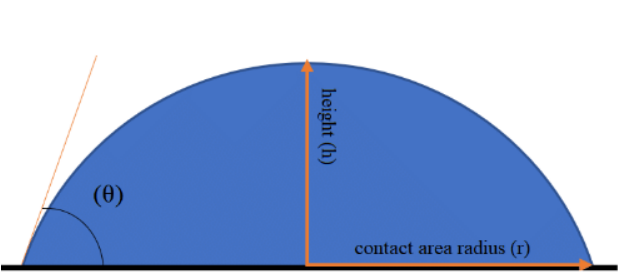
\includegraphics[width=11cm]{images/contact_angle_schematic.png}
    \caption{\label{fig:drop_geom}
    Геометрия сферической капли: $r(R_d)$ — радиус контактной области, $h$ — высота, $\theta$ — угол смачивания. Воспроизведено из работы~\cite{aboubakri2021}.}
    \end{center}
\end{figure}

Классическая формула объёма сферического сегмента имеет вид:
\begin{equation}
V = \frac{1}{3} \pi h^2 (3R - h),
\end{equation}

\[
sin\theta = \frac{R_d}{R}
\qquad
ctg\theta = \frac{R-h}{R_d}
\]

откуда $h = R(1 - \cos\theta)$.

Подставим:
\[
V = \frac{1}{3} \pi R^3 (1 - \cos\theta)^2 (2 + \cos\theta).
\]

Поскольку $R = R_d / \sin\theta$, то $R^3 = R_d^3 / \sin^3\theta$. Подставим это в выражение для $V$:
\[
V = \frac{1}{3} \pi \cdot \frac{R_d^3}{\sin^3 \theta} \cdot (1 - \cos\theta)^2 (2 + \cos\theta).
\]

Теперь введём коэффициент $B(\theta)$:
\begin{equation}
V = \frac{B(\theta)\pi R_d^3}{3}.
\end{equation}
Сравнивая, получаем:
\[
B(\theta) = \frac{\left(1-\cos\theta\right)^{2}\left(2+\cos\theta\right)}{\sin^{3}\theta}.
\]

Это выражение можно упростить до более компактной формы с использованием тригонометрических тождеств:
\[
\frac{\left(1-\cos\theta\right)^{2}\left(2+\cos\theta\right)}{\sin^{3}\theta}=\frac{\left(1-2\cos\theta+\cos^{2}\theta\right)\left(2+\cos\theta\right)}{\sin^{3}\theta}=
\]

\[
=\frac{2-4\cos\theta+2\cos^{2}\theta+\cos\theta-2\cos^{2}\theta+\cos^{3}\theta}{\sin^{3}\theta}=
\]

\[
=\frac{2-3\cos\theta+\frac{3}{4}\cos\theta+\frac{1}{4}\cos3\theta}{\frac{3}{4}\sin\theta-\frac{1}{4}\sin3\theta}=\frac{8-9\cos\theta+\cos3\theta}{3\sin\theta-\sin3\theta}
\]

\begin{equation}
B(\theta) = \frac{8-9\cos\theta+\cos3\theta}{3\sin\theta-\sin3\theta}
.
\label{eq:Btheta_final}
\end{equation}

Именно это выражение реализовано в численном коде и используется во всех вычислениях, связанных с объёмом капли.

\subsection{Рост кольца}

Рост квантового кольца происходит в результате поверхностной реакции между атомами галлия и мышьяка, приводящей к образованию кристаллической фазы GaAs. Локальное увеличение высоты кольца напрямую связано с числом образованных ячеек кристалла в данной точке.

Концентрация обоих типов атомов, связанных друг с другом и участвующих в росте кристалла, изменяется в соответствии с:

\[
\frac{dC_{\text{bound}}}{dt} = k_r \, C_{\text{Ga}}(r,t) \cdot C_{\text{As}}(r,t)
\]
где:
\begin{itemize}
  \item $C_{\text{bound}}$ — концентрация результата реакции (GaAs);
  \item $k_r$ — константа скорости реакции;
  \item $C_{\text{Ga}}, C_{\text{As}}$ — локальные концентрации атомов;
\end{itemize}

Количество вертикальных кристаллических ячеек GaAs на каждом расстоянии увеличивается в зависимости от:

\[
C_{\text{bound}} = N_{\text{cells}} \cdot C_0 \quad \Rightarrow \quad
\frac{dN_{\text{cells}}}{dt} = \frac{k_r}{C_0} \, C_{\text{Ga}} \cdot C_{\text{As}}.
\]
где:
\begin{itemize}
  \item $C_0 = \frac{1}{a_0^2}$ , $a_0$ - постоянная решётки GaAs;
  \item $N_{\text{cells}}$ — количество слоёв ячеек GaAs, выросших в данной точке (вдоль вертикали);
\end{itemize}

Высота слоя связана с этим количеством ячеек:

\[
    h=h_{0}N_{\text{cells}}
\]

\[
\frac{dh\left(r,t\right)}{dt}=\frac{h_{0}k_{r}}{C_{0}}C_{Ga}C_{As}
\]
где $h_0=a_0$ — высота одного элементарного слоя (порядка постоянной решётки);

Учитывая масштабирование концентраций с помощью $C_{0}$ и введённых параметров, мы записываем:

\[
\frac{dh\left(r,t\right)}{dt}=h_{0}C_{0}k_{r}C_{Ga}C_{As}
\]

Интегрируя это уравнение по времени, можно получить полный профиль кольца. Поскольку значения $C_{\text{Ga}}$ и $C_{\text{As}}$ варьируются по координате $r$ и времени $t$, итоговая форма кольца чувствительна к условиям роста, включая поток, температуру и геометрию капли.

\subsection{Уравнение изменения радиуса капли \texorpdfstring{$R_d(t)$}{Rd(t)}}

Изменение радиуса жидкой капли галлия во времени связано с постепенной кристаллизацией GaAs в результате взаимодействия атомов Ga и As на поверхности.
\begin{equation}
\frac{\partial C_{\text{bound}}}{\partial t}=k_{r}C_{Ga}C_{As}
\end{equation}

Это должен быть единственный способ, которым атомы Ga могут исчезнуть (за исключением тех, которые выходят за пределы границы, но мы пока отбросим их). 

Скорость изменения объёма капли пропорциональна количеству атомов, покидающих её в результате химической реакции. Если \( C_{\text{Ga}}(r,t) \) и \( C_{\text{As}}(r,t) \) — локальные поверхностные концентрации атомов галлия и мышьяка, то число атомов, вовлечённых в рост GaAs на малом интервале времени \( dt \), определяется как:

\begin{equation}
\frac{dN_{Ga}}{dt}=-2\pi k_{r}C_{0}^{2}\int_{0}^{R_{\infty}}rC_{Ga}C_{As}dr
\end{equation}

Рассмотрим сферическую каплю объёмом
\begin{equation}
V = \frac{B(\theta)\pi R_d^3}{3},
\end{equation}

Дифференцируя объём по времени, получаем:
\begin{equation}
\frac{dV}{dt} = {\pi R_d^2B(\theta)} \cdot \frac{dR_d}{dt}.
\label{eq:dVdt_from_R}
\end{equation}

С другой стороны, объём капли можно выразить через количество атомов галлия:
\begin{equation}
V = \Omega_{\text{Ga}} \cdot N_{\text{Ga}} \quad \Rightarrow \quad \frac{dV}{dt} = \Omega_{\text{Ga}} \cdot \frac{dN_{\text{Ga}}}{dt},
\label{eq:dVdt_from_N}
\end{equation}
где $\Omega_{\text{Ga}} = a_0^3$ — объём одного атома галлия.

Подставляя \eqref{eq:dVdt_from_N} в \eqref{eq:dVdt_from_R}, получаем:
\begin{equation}
\frac{dR_d}{dt} = \frac{\Omega_{\text{Ga}} }{\pi R_d^2 B(\theta)} \cdot \frac{dN_{\text{Ga}}}{dt}.
\end{equation}

Мы получаем:

\begin{equation}
\frac{dR_{d}}{dt}=-\frac{2\Omega_{Ga}k_{r}C_{0}^{2}}{B\left(\theta\right)R_{d}^{2}}\int_{0}^{R_{\infty}}rC_{Ga}C_{As}dr
\label{eq:dRdt_integral}
\end{equation}
где:
\begin{itemize}
  \item \( \Omega_{\text{Ga}} = a_0^3 \) — объём одного атома галлия;
  \item \( R_\infty \) — граница области расчёта.
\end{itemize}

При численной реализации интеграл в уравнении \eqref{eq:dRdt_integral} заменяется на дискретную сумму по координатной сетке, как будет показано в главе 3. Тем не менее, приведённая здесь непрерывная форма демонстрирует физическую суть: скорость уменьшения радиуса капли определяется пространственно распределённой реакцией атомов Ga и As на поверхности.

% ============================================
% ГЛАВА 2
% ============================================
\pagebreak
\section{Теория и основные уравнения}

\subsection{Раздел 1}

Ненумерованная формула:

\begin{equation}
    \begin{pmatrix} \dot{\varphi}\\ \dot{\theta} \\ \dot{\psi} \end{pmatrix}
    = \begin{pmatrix}
        \cos(\theta)\cos(\psi) & -\sin(\psi) & 0 \\
        \cos(\theta)\sin(\psi) & \cos(\psi)  & 0 \\
        -\sin(\theta)         & 0         &  1
    \end{pmatrix}^{-1}
    \begin{pmatrix} \omega_x\\ \omega_y \\ \omega_z \end{pmatrix}. \nonumber
\end{equation}


\begin{equation}
    E_{y}\left(z\geq L\right)=A_{12}e^{i\beta z}\cdot\begin{cases}
        e^{sw}\cos\left(kw\right)e^{s\left(x-a\right)}, & x<a-w\\
        \cos\left(k\left(x-a\right)\right), & a-w\leq x\le a+w\\
        e^{sw}\cos\left(kw\right)e^{-s\left(x-a\right)}, & x>a+w
        \end{cases}    
\end{equation}


\subsection{Раздел 2}

Нумерованные формулы:

\begin{equation}
\label{eq:1}
    \dot{\theta}=\frac{P-p_{1}\cos\left(\varphi_{1}-\theta\right)-p_{2}\cos\left(\varphi_{2}-\theta\right)}{\mu+\sin^{2}\left(\varphi_{1}-\theta\right)+\sin^{2}\left(\varphi_{2}-\theta\right)}
\end{equation}

\begin{equation}
    \dot{\varphi}_{1}=p_{1}-\dot{\theta}\cos(\phi_{1}-\theta)
\end{equation}

\begin{equation}
    \dot{\varphi}_{2}=p_{2}-\dot{\theta}\cos(\phi_{2}-\theta)
\end{equation}

Тест ссылки на формулу (\ref{eq:1}).

% ============================================
% ГЛАВА 3
% ============================================
\pagebreak
\section{Численные методы и алгоритмы}

\subsection{Раздел 1}

\subsection{Раздел 2}

\begin{lstlisting}[language=rust,caption={Программная реализация метода Рунге-Кутты},label={listing-1}]
    // From the pendulum program
    fn runge_kutta(
        vars: &MyVec,
        pars: &Vec<f64>,
        rhs: &dyn Fn(&MyVec, &Vec<f64>) -> MyVec,
        dt: f64,
    ) -> MyVec {
        let rk_1 = rhs(vars, pars);
        let rk_2 = rhs(&vars.add(&rk_1.scale(dt / 2.0)), pars);
        let rk_3 = rhs(&vars.add(&rk_2.scale(dt / 2.0)), pars);
        let rk_4 = rhs(&vars.add(&rk_3.scale(dt)), pars);
    
        let vars_new = vars
            .add(&rk_1.scale(dt / 6.0))
            .add(&rk_2.scale(dt / 3.0))
            .add(&rk_3.scale(dt / 3.0))
            .add(&rk_4.scale(dt / 6.0));
        vars_new
    }
    \end{lstlisting}
    
    \begin{lstlisting}[language=C++,caption={Подпрограмма случайного блуждания на плоскости},label={listing-2}]
    std::random_device rd;
    std::mt19937 mt(rd());
    std::uniform_int_distribution<long> dist(1, 4);
    std::vector<long> xn(n0, 0);
    std::vector<long> yn(n0, 0);
    for (long jt = 0; jt < M; jt++)
    {
        for (long jn = 0; jn < n0; jn++)
        {
            switch (dist(mt))
            {
            case 1:
                xn[jn] ++;
                break;
            case 2:
                xn[jn] --;
                break;
            case 3:
                yn[jn] ++;
                break;
            case 4:
                yn[jn] --;
                break;
            }
        }
    }
\end{lstlisting}

% ============================================
% ГЛАВА 4
% ============================================
\pagebreak
\section{Результаты и обсуждение}

В начало надо поместить описание использованных в расчётах материалов, моделей и параметров, а также обоснование выбора (детальный обзор параметров из литературы можно поместить в главу с теорией или даже в обзор).

Таблицы в \LaTeX ~делать очень неудобно. Лучше воспользоваться сторонним редактором таблиц, которые умеет их экспортировать в \LaTeX, сделать там всю структуру, а потом вставить готовый код, и в нём уже добавлять содержимое ячеек.

Тем не менее, простые таблицы делать можно, наподобие \ref{table-1}. Но лучше таблицами вообще не злоупотреблять, а где можно заменять их графиками и диаграммами.

\begin{center}
\begin{table}[h]
\centering{}%
\caption{Условия роста образцов с квантовыми кольцами\label{table-1}}
\begin{tabularx}{0.9\textwidth}{|B|R|R|R|R|R|X|X|}
\hline 
№ & $X_{\text{In}}$, \% & $T_1$, °C & $T_2$, °C & $P_{\text{As}_4}$, $10^{-5}$ Торр & Тип КК & \multicolumn{2}{R|}{Диаметры, нм} \tabularnewline
\hline
А1 & 0 & 220 & 220 & 1,3 & Одиночное & \multicolumn{2}{R|}{51} \tabularnewline
\hline
А2 & 0 & 280 & 280 & 0,55 & Двойное & 120 & 42 \tabularnewline
\hline
Б1 & 5 & 250 & 250 & 5,0 & Одиночное & \multicolumn{2}{R|}{75}  \tabularnewline
\hline 
Б2 & 10 & 250 & 250 & 5,0 & Одиночное & \multicolumn{2}{R|}{76}  \tabularnewline
\hline 
Б3 & 20 & 250 & 250 & 5,0 & Одиночное & \multicolumn{2}{R|}{78}  \tabularnewline
\hline 
Б4 & 20 & 200 & 200 & 5,0 & Одиночное & \multicolumn{2}{R|}{63}  \tabularnewline
\hline 
В1 & 0 & 325 & 325 & 0,2 & Одиночное & \multicolumn{2}{R|}{22}  \tabularnewline
\hline 
В2 & 0 & 325 & 220 & 0,2 & Двойное & 79 & 31 \tabularnewline
\hline 
В3 & 0 & 325 & 325 & 1,0 & Двойное & 69 & 27 \tabularnewline
\hline
\end{tabularx}
\end{table}
\end{center}

Ссылаемся на Листинг \ref{listing-1} здесь.

% ============================================
%  ВЫВОДЫ И ЗАКЛЮЧЕНИЕ
% ============================================
\pagebreak
\specialsection{Выводы}
Структура файлов, которые можно редактировать:

\begin{itemize}
    \item \verb|diploma.tex| --- содержит основной текст;
    \item \verb|titlepage.tex| --- содержит титульный лист;
    \item \verb|literature.bib| --- содержит источники для списка литературы;
    \item \verb|code_highlight.tex| --- форматирование листингов (фрагментов кода).
\end{itemize}

Файл \verb|style.tex| очень важный, его трогать и особенно удалять не надо, там задаются различные стили документа. Редактировать в случае, если знаете, что делать.

\specialsection{Заключение}

Нужны ли отдельно и выводы, и заключение --- я не знаю. Разберёмся.

Список литературы ниже оформлен не совсем по ГОСТу, но это легко исправить. Главное, что он организован, и можно ссылаться на каждый пункт по фамилии первого автора.

\textbf{Внимание!} 

Список литературы находится в отдельном файле \verb|literature.bib|, в который можно добавлять новые источники в любом порядке. Они будут сами располагаться как нужно, в порядке упоминания в тексте.

Если какой-то источник не процитирован в тексте, он в список литературы добавлен не будет.

Поэтому один и тот же файл с источниками можно использовать для нескольких документов.


\pagebreak
\printbibliography

\end{document}
